\documentclass[12pt,prb,aps,epsf]{article}
\usepackage[utf8]{inputenc}
\usepackage{amsmath}
\usepackage{amsfonts}
\usepackage{amssymb}
\usepackage{graphicx} 
\usepackage{latexsym} 
\usepackage[toc,page]{appendix}
\usepackage{listings}
\usepackage{xcolor}
\usepackage{soul}
\usepackage[T1]{fontenc}
\usepackage{amsthm}
\usepackage{mathtools}
\usepackage{setspace}
\usepackage{array,multirow,makecell}
\usepackage{geometry}
\usepackage{textcomp}
\usepackage{float}
%\usepackage{siunitx}
\usepackage{cancel}
%\usepackage{tikz}
%\usetikzlibrary{calc, shapes, backgrounds, arrows, decorations.pathmorphing, positioning, fit, petri, tikzmark}
\usepackage{here}
\usepackage{titlesec}
%\usepackage{bm}
\usepackage{bbold}

\geometry{hmargin=2cm,vmargin=2cm}

\begin{document}
	
	\title{MP 26 Mesure de longueur}
	\author{Naïmo Davier}
	\date{Agrégation 2019}
	
	\maketitle
	
	\tableofcontents
	
	\pagebreak
	
\section{Parallaxe}
On va illustrer le principe de la parallaxe en mesurant la distance entre un plan contenant deux goniomètres et un point/fente source. Voir le \textbf{Bélier}.\\ 
On réalise donc tout d'abord une mesure de cette distance $h$ à l'aide d'un mètre ruban, afin d'avoir une valeur à comparer.\\
On mesure maintenant la distance séparant les centres (de rotation) des deux goniomètres, notée $d$.
\begin{figure}[h]
	\centering 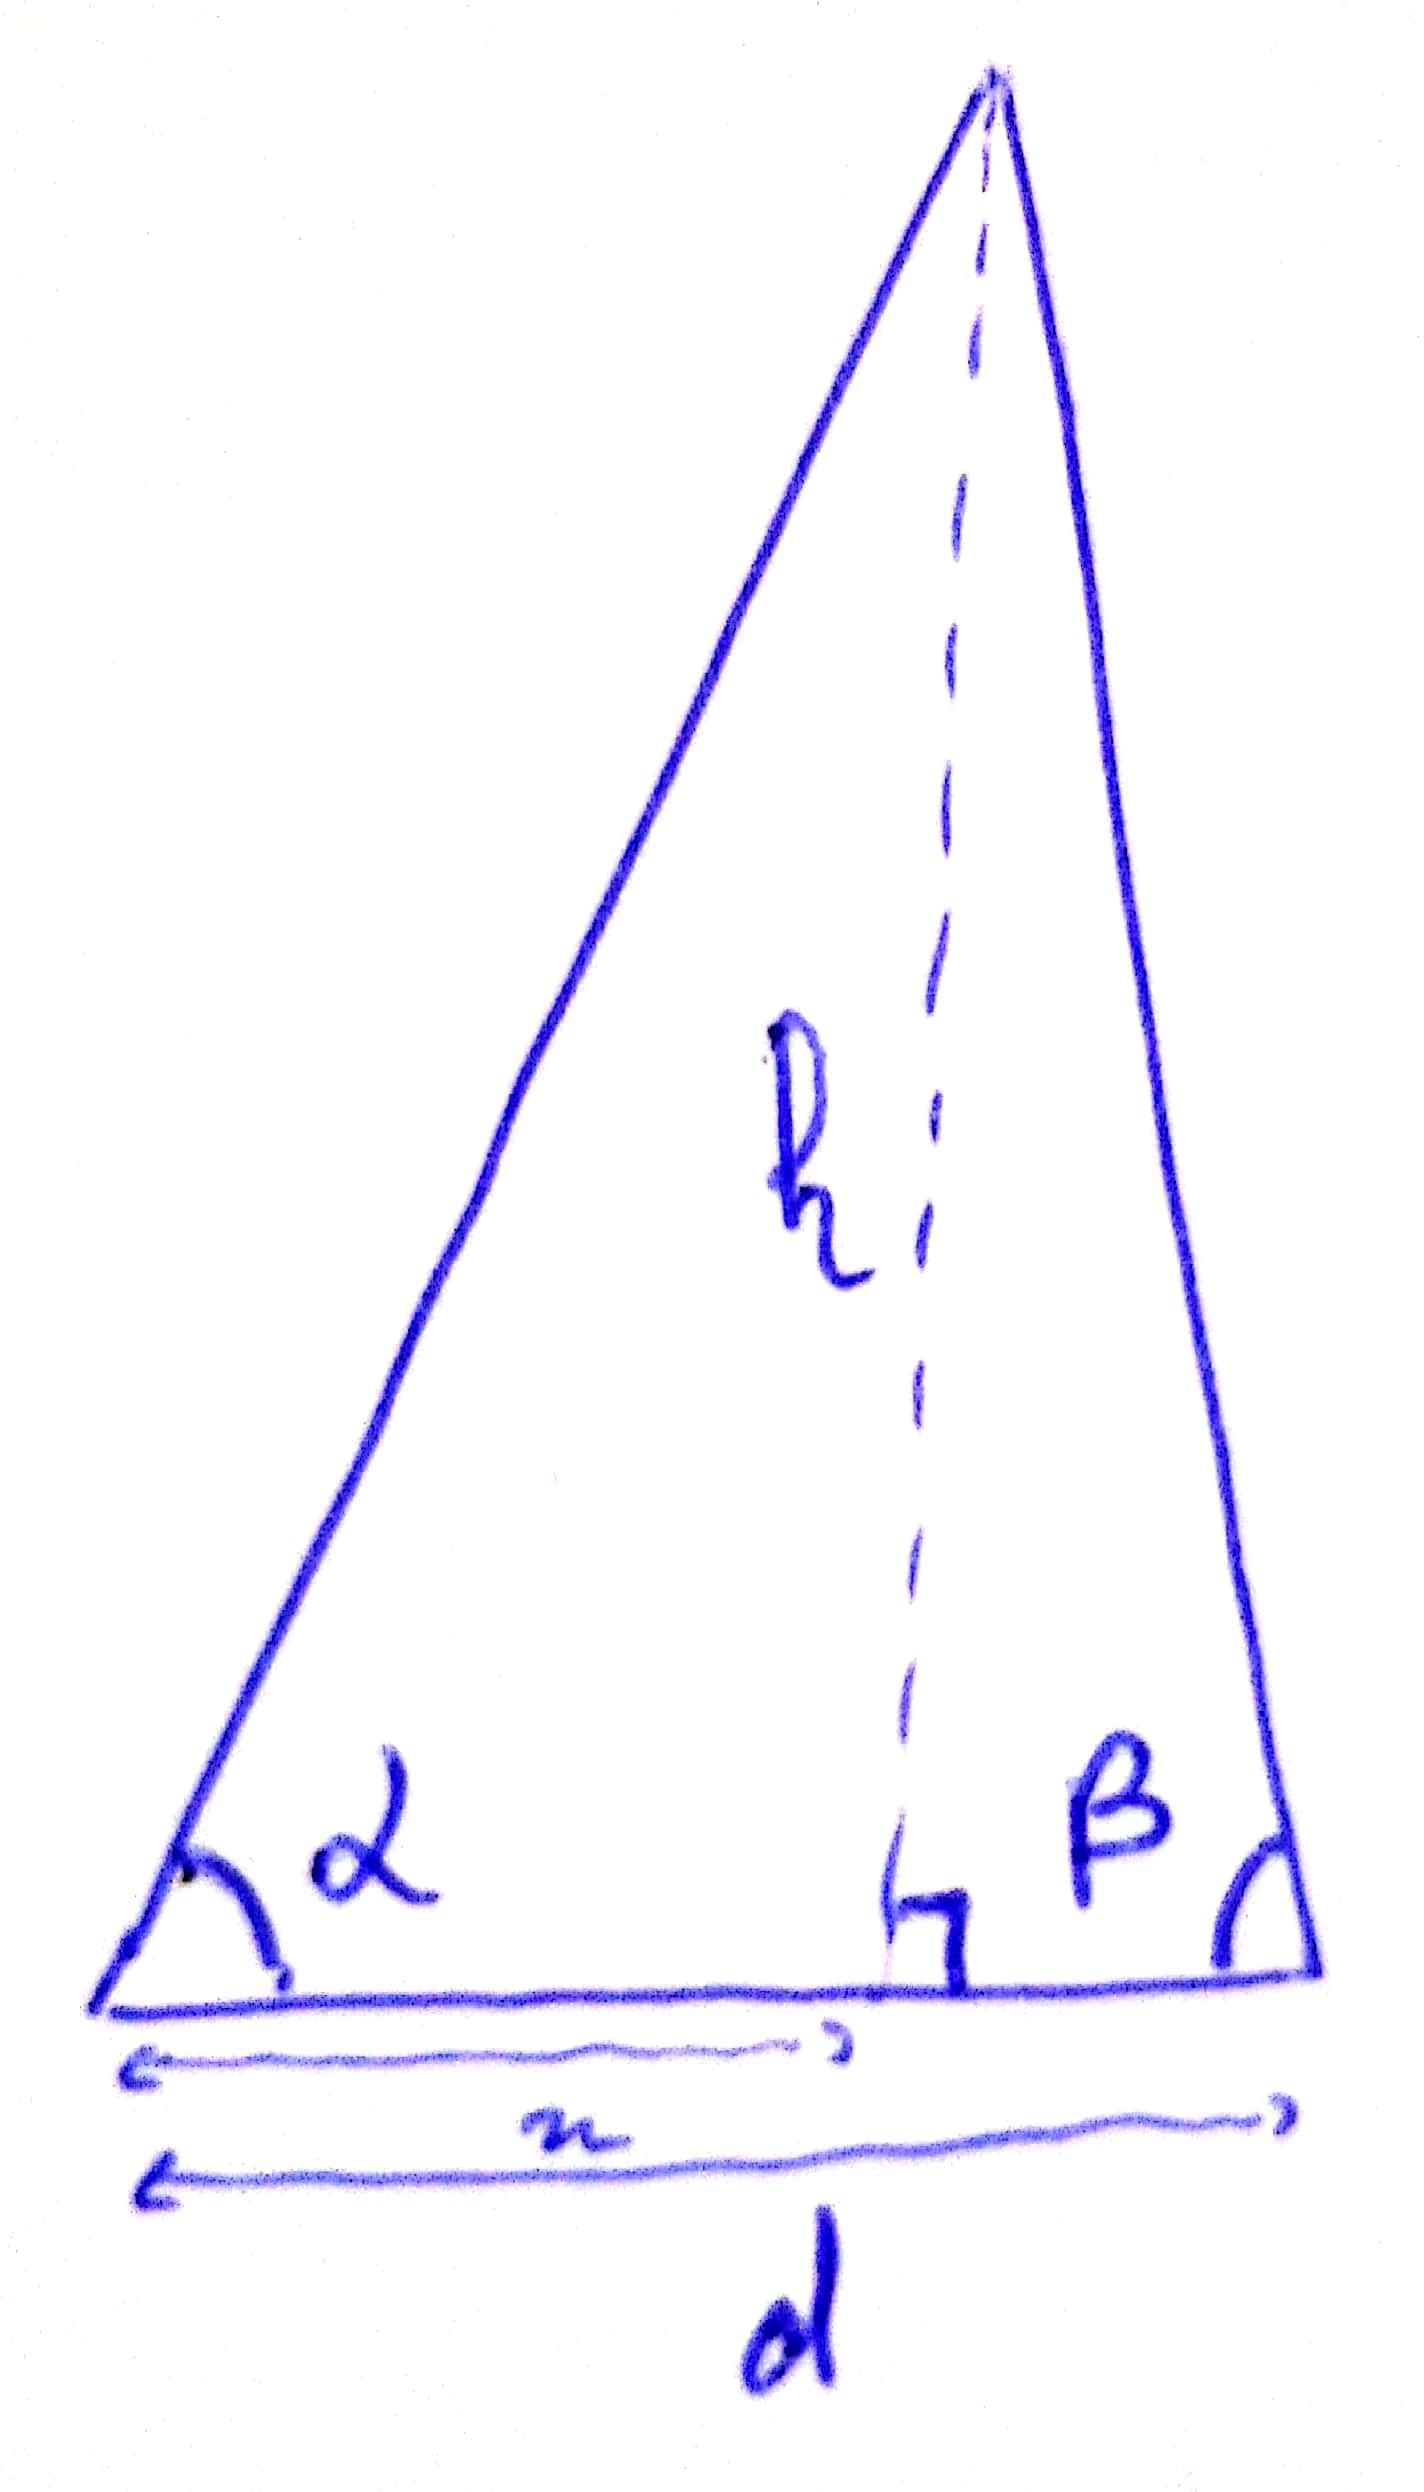
\includegraphics[width=5cm]{parallaxe}
\end{figure}
On définit ensuite un angle de référence pour chacun des gonio en pointant le réticule de l'autre gonio, qu'on aura pris le soin d'éclairer avec la lumière interne à l'oculaire. On mesure ensuite les angles $\alpha$ et $\beta$ tels que représentés sur la figure, en estimant au passage les incertitudes associées. On en déduit alors une mesure de $h$ selon 
\begin{eqnarray}
\tan\alpha = \frac{h}{x}\hspace{1cm}&\mathrm{et}&\hspace{1cm} \tan \beta = \frac{h}{d-x}\\
&\Longrightarrow& \frac{h}{\tan \alpha} = d - \frac{h}{\tan \alpha}\\
&\Longrightarrow& h = \frac{d}{\frac{1}{\tan\alpha} + \frac{1}{\tan\beta}}
\end{eqnarray}

Pour ce qui est de l'estimation des incertitudes, on peut, pour s'éviter des calculs trop pénibles, considérer que 
\begin{eqnarray}
\frac{u(\alpha)}{\alpha} \simeq \frac{u(\beta)}{\beta}
\end{eqnarray}
et estimer l'incertitude dans le cas simple où on a un placement symétrique des goniomètres et ainsi $\alpha \simeq \beta$. On a alors 
\begin{eqnarray}
h \simeq \frac{d \tan\alpha}{2}
\end{eqnarray}
et ainsi, en appliquant la formule générale pour une une fonction $h(d, \alpha)$
\begin{eqnarray}
u(h)^2 = \left(\frac{\partial h}{\partial \alpha}u(\alpha)\right)^2 + \left(\frac{\partial h}{\partial d}u(d)\right)^2
\end{eqnarray}
on obtient 
\begin{eqnarray}
u(h)^2 &=& \frac{d^2}{4}(1+\tan^2\alpha)u(\alpha)^2 + \frac{\tan^2\alpha}{4}u(d)^2\\
\frac{u(h)^2}{h^2} &=& \frac{u(d)^2}{d^2} + \frac{u(\alpha)^2}{\sin^2\alpha}
\end{eqnarray}
on peut alors estimer l'incertitude relative sur $h$ assez facilement. Dans la pratique $u(\alpha)$ est en radiant et donc une valeur très petite : l'incertitude sur la mesure des angles sera négligeable devant celle sur la mesure de $d$.\\

Ce protocole peut se révéler laborieux quand à l'alignement des gonio et la mesure de l'angle de référence correspondant. On peut donc appliquer une méthode équivalente sur le principe mais peut être plus évidente à réaliser : on place la fente source d'un des deux gonio (munie d'une lampe) sur l'axe liant les deux gonio, puis on aligne les deux oculaires par rapport à cette fente pour définir les angles de références.\\

Ne pas oublier de bien régler les oculaires :  la lentille coté œil doit être réglée de telle sorte à voir le réticule net, et la seconde lentille (coté objet) doit être réglée de telle sorte à former l'image d'un objet à l'infini dans le plan focal objet de la première lentille (et donc dans le même plan que le réticule). 

\section{Effet piezo électrique}
On va utiliser un interféromètre de Michelson pour mesurer de combien se dilate un petit piezo en fonction de la tension qu'on lui impose.\\

On commence par régler un Michelson à l'aide d'un laser (dont la longueur d'onde doit être choisie en accord avec la photodiode, et mesurée au spectro pour lever l'incertitude du constructeur), et en se plaçant proche du contact optique.\\ 
On place alors un piezo entre le bras sur lequel on charriote et le miroir, puis on se replace proche du contact optique.\\ 
On place maintenant une photodiode devant le michelson, et on la relie à la deuxième entrée d'un oscillo.\\
On connecte maintenant le piezo à une alimentation courant tension délivrant deux sorties à $0-30$ V, et on relie la borne + d'une sortie à la borne - de l'autre pour avoir un générateur délivrant une tension dans la plage 0-60 V. On regardera la tension aux bornes du piezo sur la sorte 1 de l'oscillo.\\

On place maintenant l'oscillo en mode XY, puis en mode persistance $\infty$ (dans display), on verra alors une sinusoïde se tracer lorsqu'on fera passer la tension appliquée au piezo de 0 à 60 V, correspondant au passages de franches lumineuses devant la photodiode. \\
L'oscillo ne permettant que de visualiser une plage de 40 V on fera un pont diviseur de tension divisant par deux la tension lue par l'oscillo.\\

On relèvera maintenant l'abscisse en tension du énième pic, pour cela il est plus précis de se replacer en affichage temporel pur identifier quand est ce que $V_{diode}$ est max. On tracera alors 
\begin{eqnarray}
n = f(V_n),
\end{eqnarray}
courbe que l'on modélisera par une droite $n = aV_n + b$. Or on sait que le fait de voir passer une frange devant la diode signifie que l'on a dilaté de piezo d'une demie longueur d'onde (la lumière se réfléchie sur le miroir et fait donc un aller retour: cela engendre une différence de chemin optique de $\lambda$). Cela signifie que le piezo se dilate en fonction de la tension qui lui est appliquée comme 
\begin{eqnarray}
\delta l = a\frac{\lambda}{2}V
\end{eqnarray}
(on aura vérifié que $b$ est compatible avec le zéro.)
on pourra alors comparer le coefficient $a\frac{\lambda}{2}$ à celui donné par la doc.\\

\textbf{Remarque} : la photodiode fonctionne comme un générateur de courant, il faut ainsi convertir ce courant en tension pour réaliser notre mesure, cela se fait en mettant une résistance en série et en prenant la tension à ces bornes (ce dispositif ne doit pas être réalisé : il est déjà réalisé dans le boitier contenant la photodiode).

\section{Réflexion d'ultrasons}
On dispose d'un émetteur et d'un récepteur ultrasons, ayant un fonctionnement optimal pour 40,5 kHz environ. On va observer le signal réfléchis sur un écran (en bois de préférence : forme plus régulière du signal réfléchi) et en déduire la distance à cet écran.\\

On commence par façonner le signal que l'on va émettre : on prend deux sorties d'un GBF Rigol ou deux GBF, l'un envoyant un signal carré de fréquence comprise entre 10 et 100 Hz, l'autre une sinusoïde oscillant à la fréquence optimale pour l'émetteur ultrason(40,5 kHz). On multiplie ensuite ces deux signaux pour former des trains d'onde, l'écart $\Delta t$ entre les fronts de l'onde envoyée et de l'onde reçue nous donne alors la distance de l'écran à un plan contenant les détecteurs en connaissant la vitesse du son dans l'air à la température de la pièce. On prendra 343,4 m/s pour 20°C, sachant que cette vitesse varie de 3 m/s pour 5°C. On en déduit alors 
\begin{eqnarray}
L = c\Delta t
\end{eqnarray}
et ainsi 
\begin{eqnarray}
h^2 = \frac{L^2}{4} - \frac{d^2}{4} = \frac{c_s^2\Delta t^2}{4} - \frac{d^2}{4} 
\end{eqnarray}
avec $L$ la longueur du trajet effectué par l'onde réfléchie, $h$ la distance du plan contenant l'émetteur et le récepteur à l'écran et $d$ la distance entre l'émetteur et le récepteur.

\begin{figure}[h]
	\centering 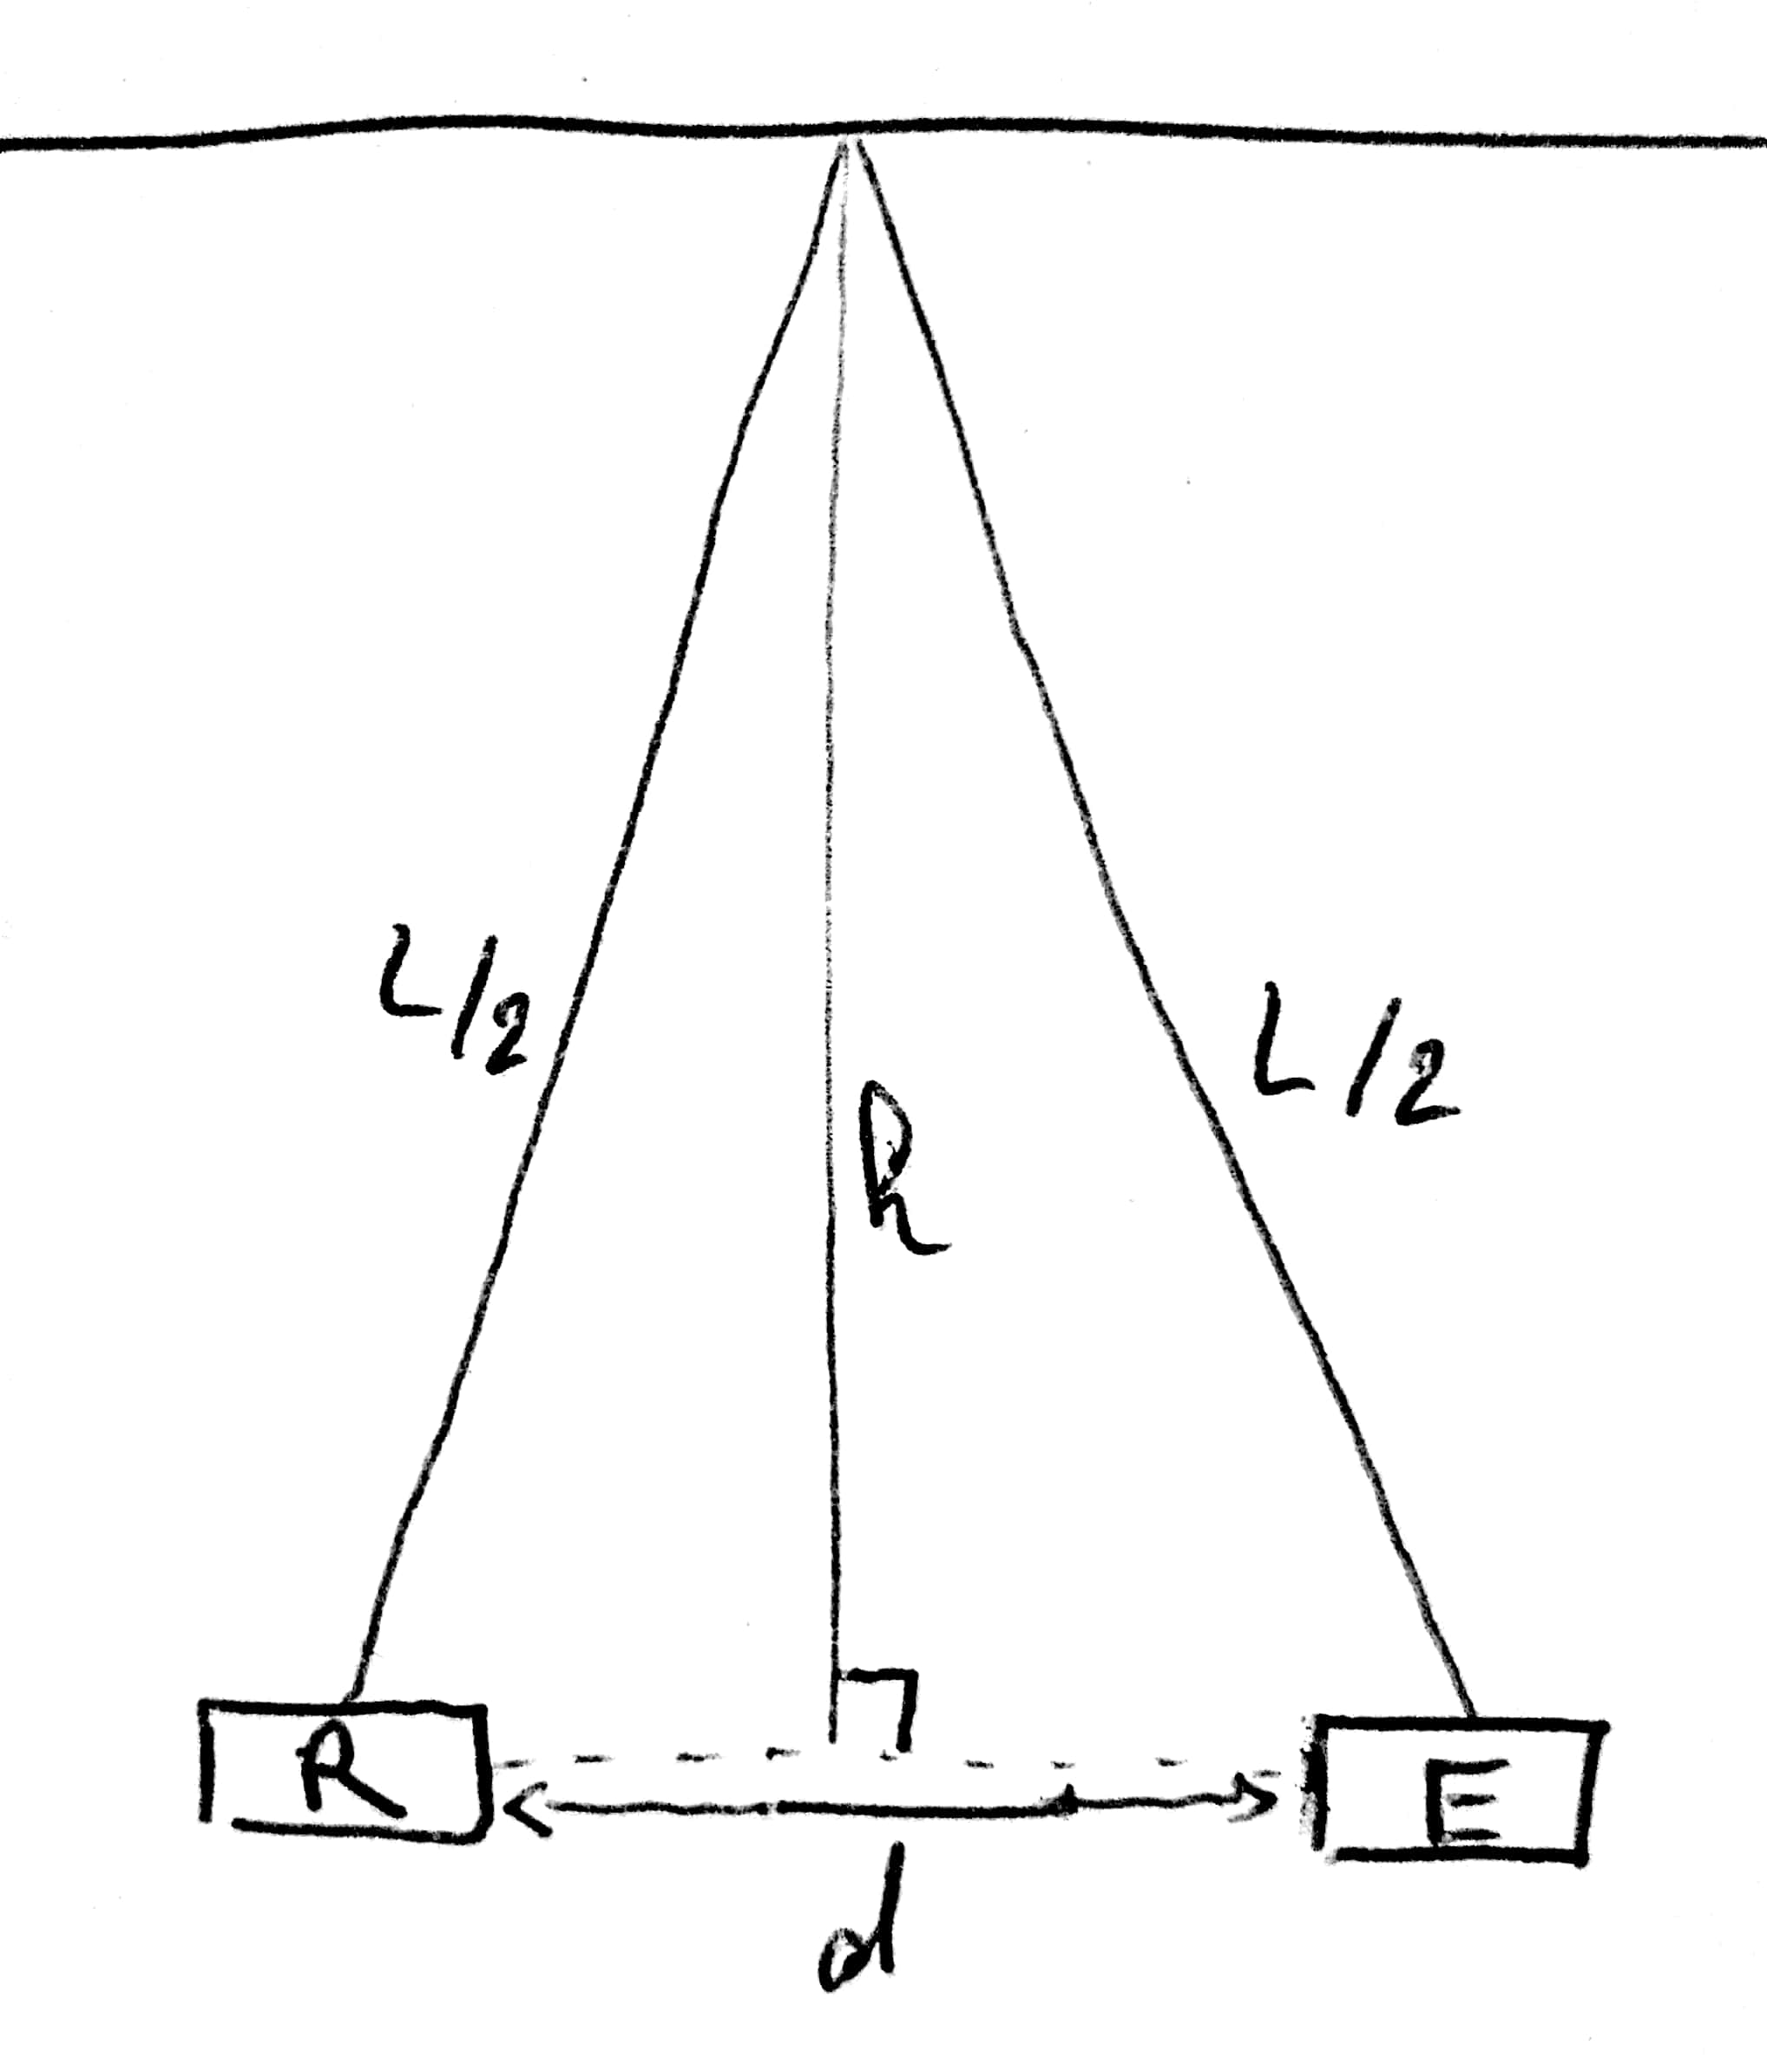
\includegraphics[width=6cm]{reflection}
				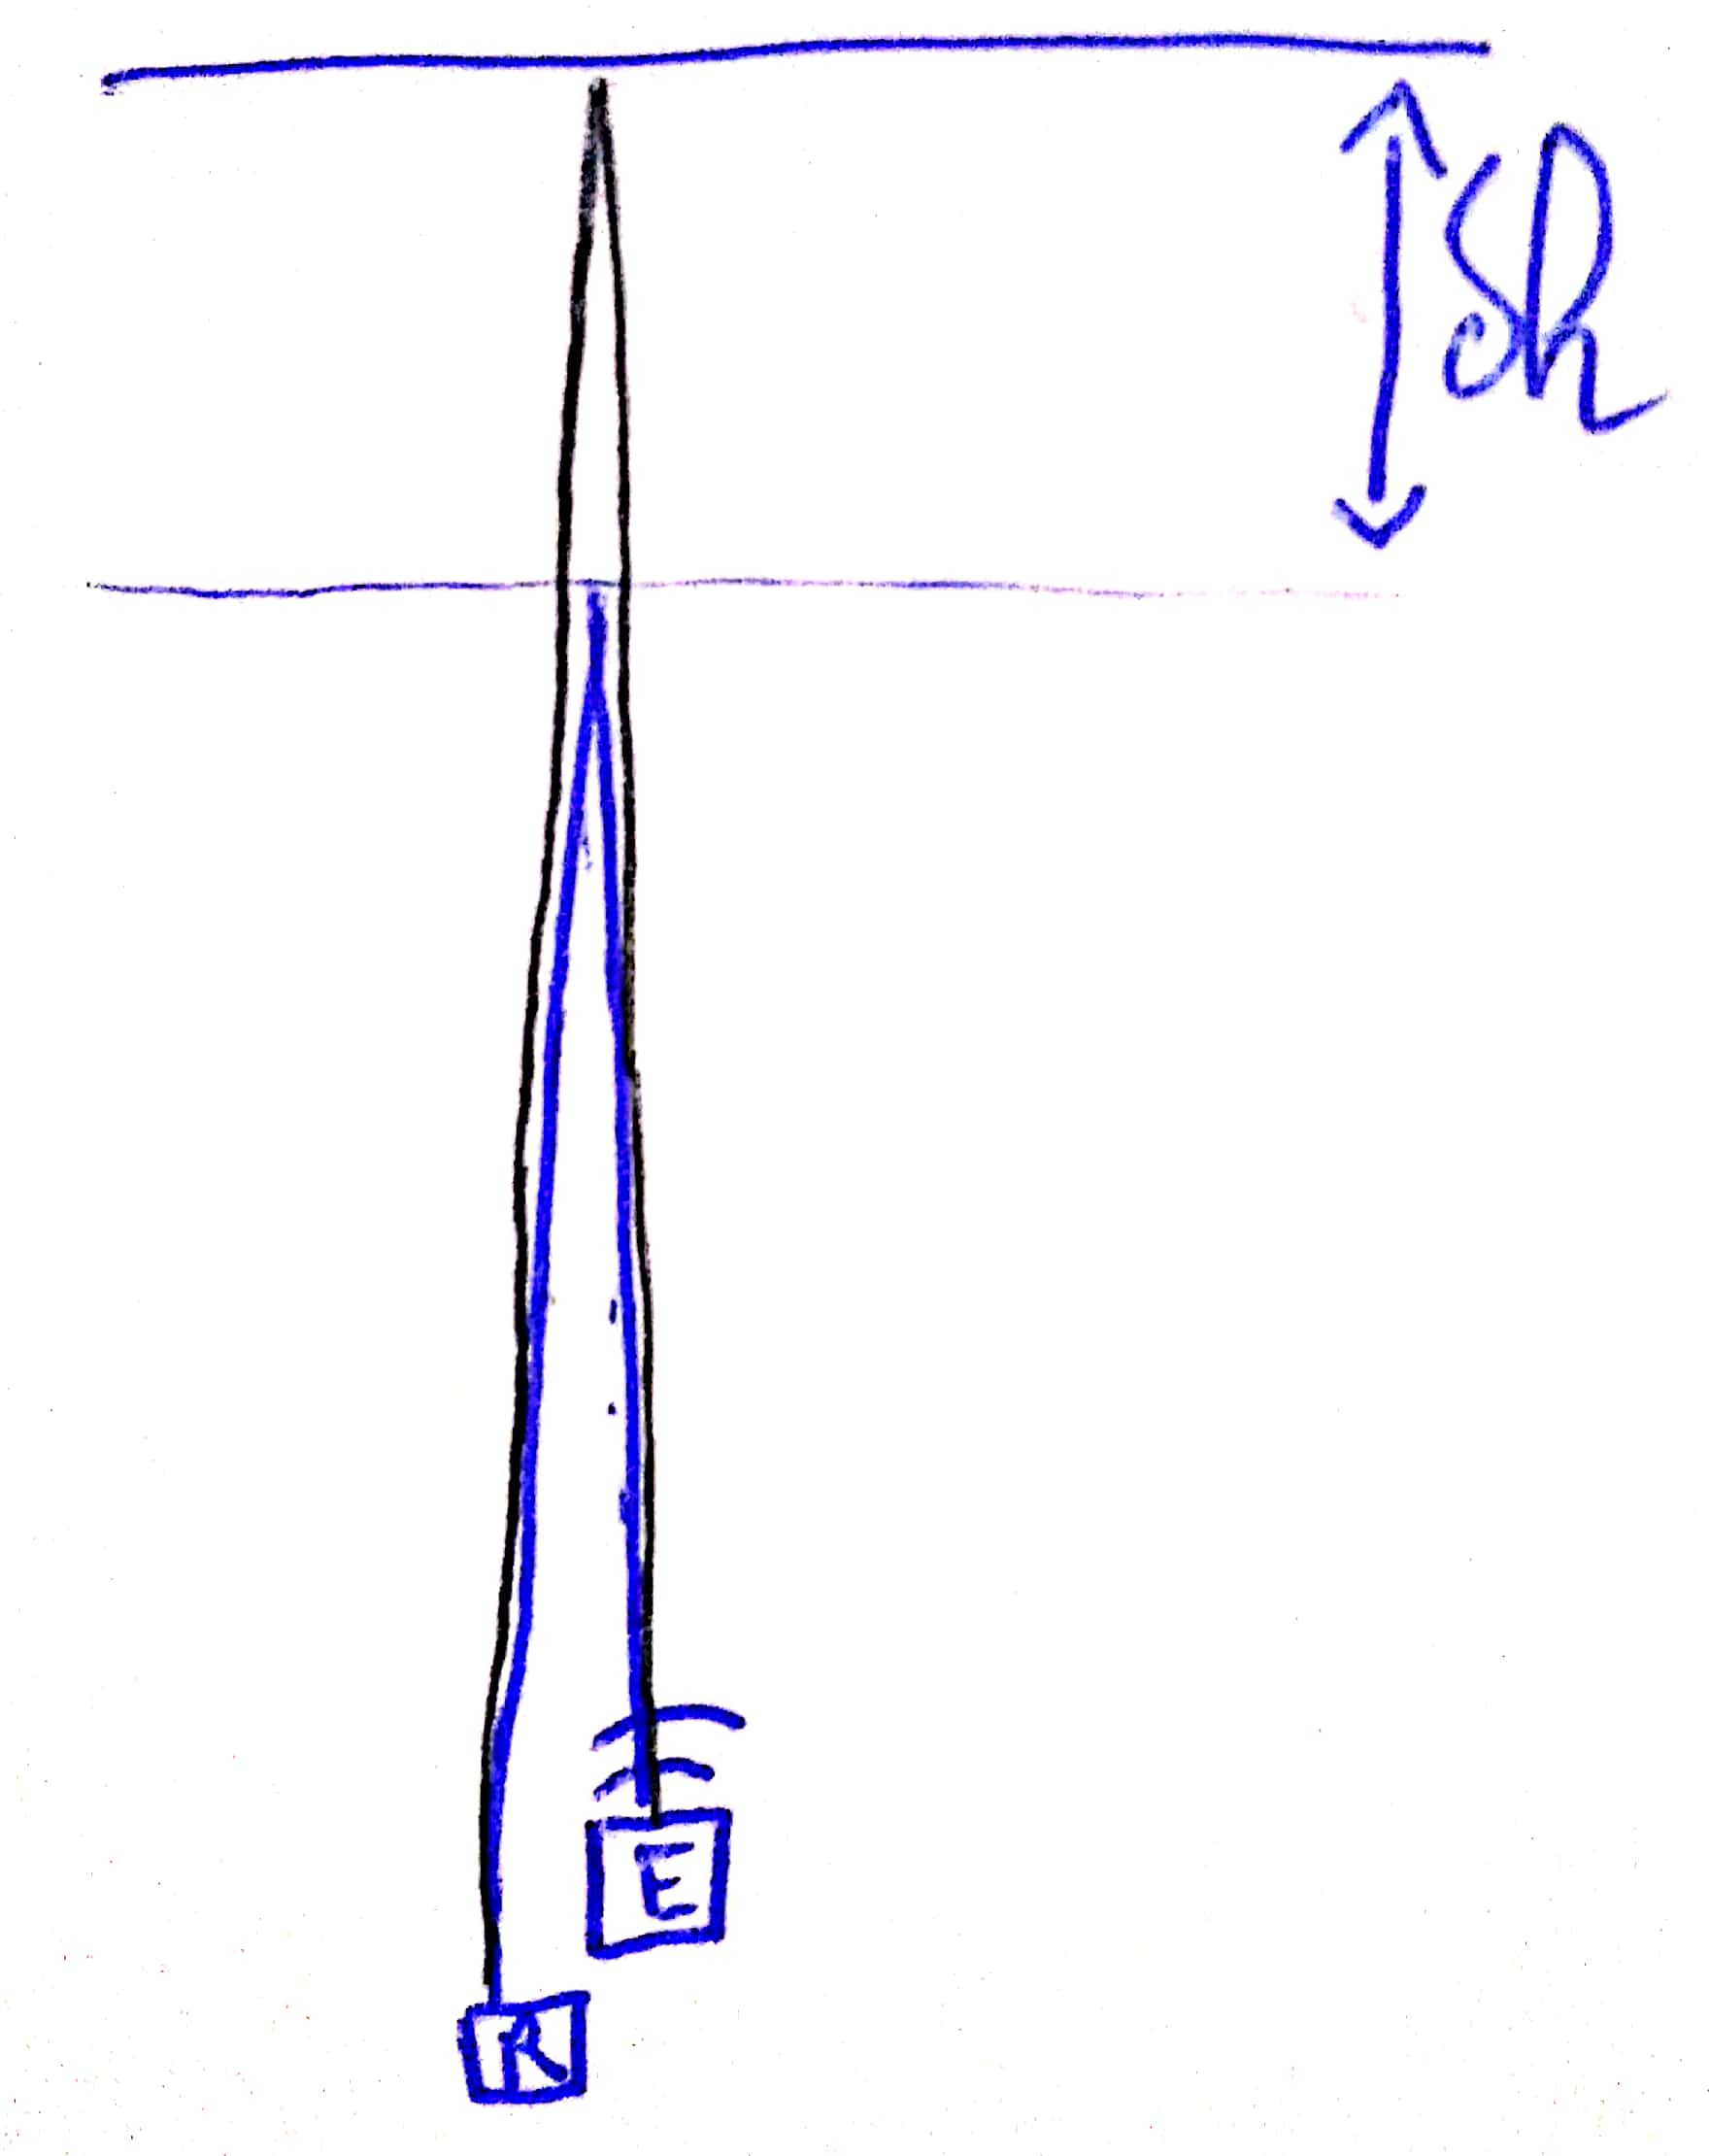
\includegraphics[width=5cm]{differentielle}
\end{figure}

Le problème de cette manip est d'identifier la position du front de l'onde réfléchie, ce qui mène à une grosse incertitude. Pour s'en affranchir on peut placer l'émetteur devant le récepteur, juste un petit peu décalé, puis faire deux mesures successives en déplaçant l'écran. Dans ce cas le choix de protocole utilisé pour repérer le front n'impacte pas la mesure, puisqu'on utilise le même pour les deux mesures. Dans ce cas on ne mesure cependant que la distance dont l'écran a été déplacé, qui vaudra alors environ 
\begin{eqnarray}
\delta h \simeq \frac{c_s \Delta t}{2}
\end{eqnarray}


Le résultat obtenu n'est pas très précis : on fait une mesure à quelques \%.\\ 
Pour améliorer le résultat on peut faire $N$ mesures en préparation pour $t_1$, puis ainsi faire diviser l'incertitude obtenue par $\sqrt{N}$. On déplacera alors l'écran en direct puis on fera de même pour $t_2$ : on obtient ainsi une meilleur incertitude pour $\Delta t$.\\
L'autre problème provient de la méconnaissance de $c_s$ qui dépend de l'hydrométrie en plus de la température, on peut donc utiliser l'émetteur et le récepteur pour mesurer la longueur d'onde et en déduire une mesure de $c_s$, cf montage n°29 (on le fera en préparation et non en direct).


\end{document}